\begin{figure}[hbt!]
\chapter{製作過程}
\end{figure}
\section{建立機器人}
\begin{figure}[hbt!]
\begin{center}
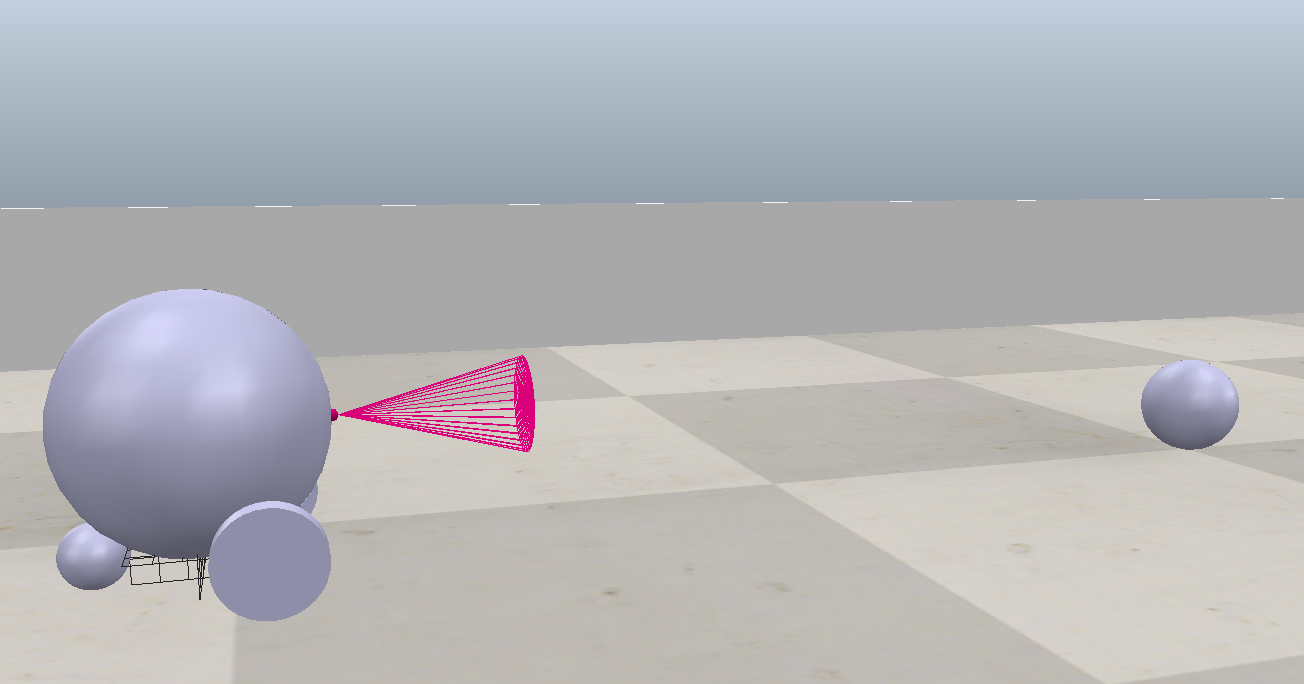
\includegraphics[width=16cm]{車車}
\caption{\Large 泡泡機器人}\label{泡泡機器人}
\end{center}
\end{figure}
\fontsize{14pt}{2.5pt}\sectionef
泡泡機器人的製作過程,首先先新增球體當作機器人主體,接下來新增兩軸當作馬達,然後分別裝上車輪,再來新增感測器,這時的機器人後面沒有支撐,所以我們在後面新增滑塊,車體就能保持平衡,這就是我們的泡泡機器人,詳細wink可以到\\
https://mdecd2023.github.io/2a-pj1ag5/content/tutorial1.html \\
\newpage
\section{建立球框}
\begin{figure}[hbt!]
\begin{center}
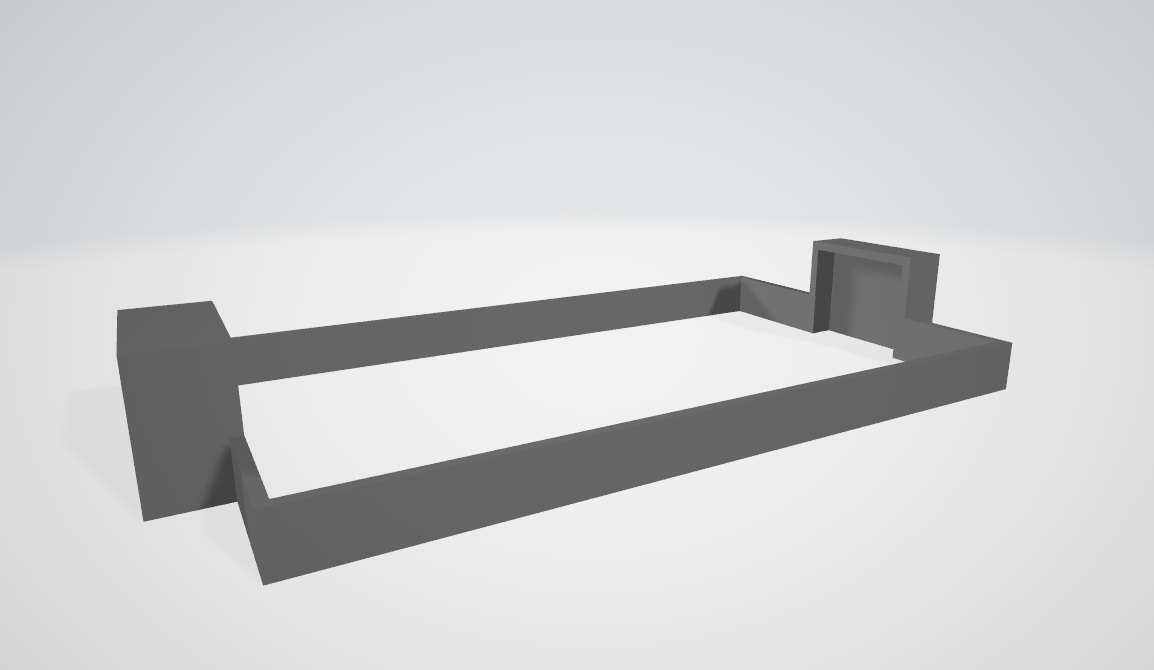
\includegraphics[width=16cm]{球框}
\caption{\Large 球框}\label{球框}
\end{center}
\end{figure}
球門我們利用NX來製作,這裡就不詳細說明,可以到\\
https://mdecd2023.github.io/2a-pj1ag5/content/project1.html\\
了解詳細過程 \\
\newpage
\section{程式}
\begin{figure}[hbt!]
\begin{center}
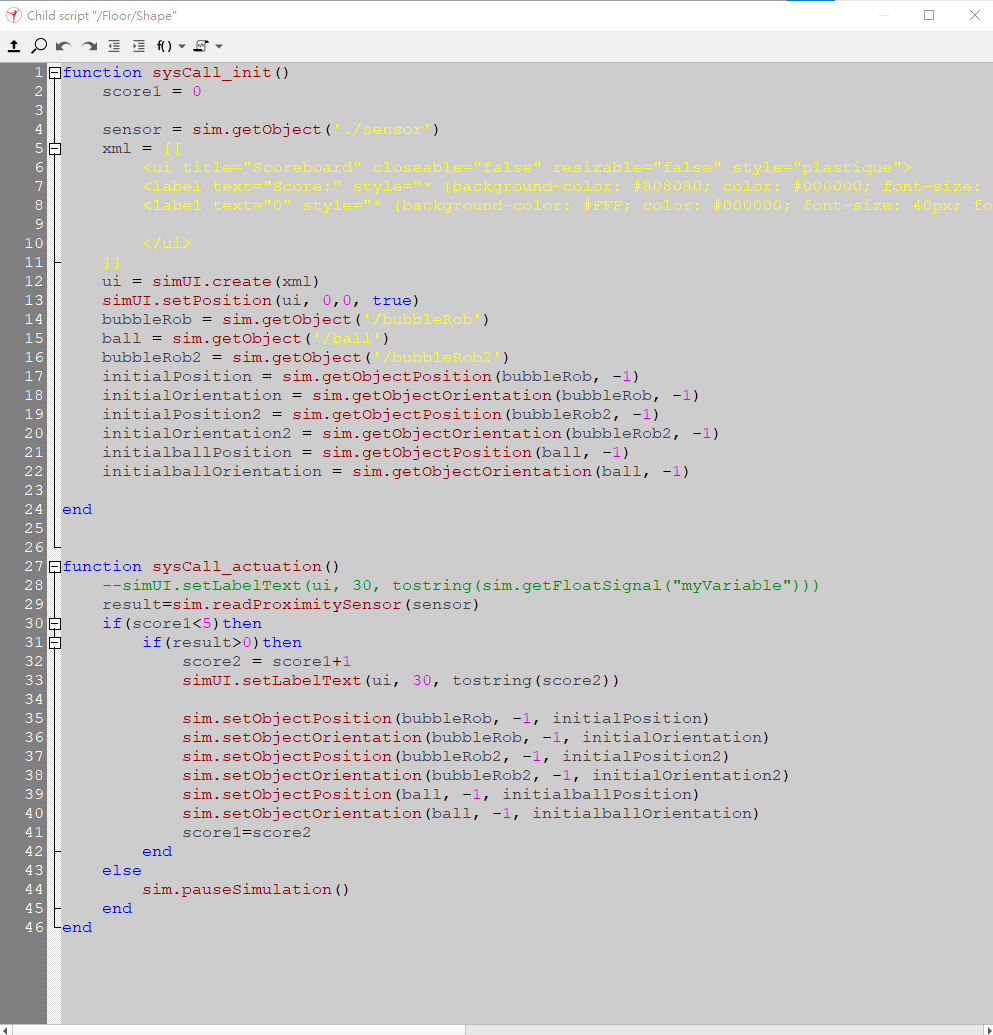
\includegraphics[width=16cm]{程式}
\caption{\Large 程式}\label{程式}
\end{center}
\end{figure}
關於程式的講解,這裡就不詳細說明,可以到\\
https://mdecd2023.github.io/2a-pj1ag5/content/project1.html\\
了解詳細過程 \\
\newpage
